\section{Introduction}%
\label{sec:Intro}
An ideal diatomic gas has two more means of storing energy compared to the
monotonic case: vibrational and rotational. Strictly speaking vibrational and
rotational modes are coupled and rotational-electronic and are coupled. However,
there are cases where this can be ignored and others where reality requires a
more nuanced quantum mechanic approach. One important assumption we will be
making is the \textbf{Born-Oppenheimer approximation}. This simply states that
electronic movement occurs on a timescale where nuclei are effectively
stationary. Therefore, we can solve the Schrödinger equation for the electrons
with stationary nuclei and for nuclei in an electron cloud. The interatomic
interactions determined by the electron cloud often is difficult to solve so
empirical and semi-empirical potentials like \textbf{Moore} or
\textbf{Leonard-Jones} are often used. Figure~\ref{fig:diatomicpotential} shows
an experimentally determined interatomic potential with a dashed line
representing the Moore's potential.
\begin{figure}[htpb]
	\centering
	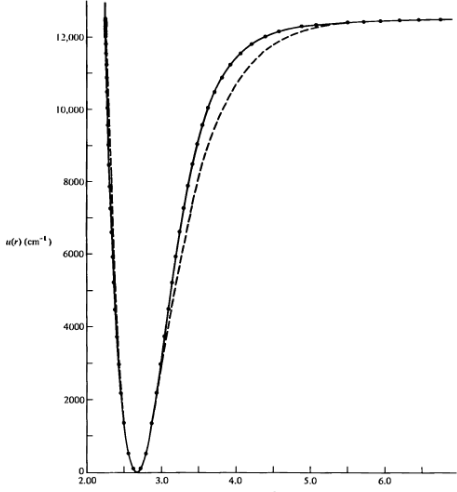
\includegraphics[width=0.6\linewidth]{interatomic_potential.png}
	\caption{Interatomic potential of a diatomic species.}
	\label{fig:diatomicpotential}
\end{figure}

\section{Rigid Rotor Harmonic Oscillator}%
\label{sec:RR}
For a diatomic atom, we first notice we can define translational movement as
that movement with respect to the center of mass, thus the Hamiltonian becomes
\begin{equation*}
	\mathcal{H} = \mathcal{H}_{trans} + \mathcal{H}_{int},
\end{equation*}
where the second term is the energy from the relative motion of the two masses.
This relative motion is clearly either rotational or vibrational. Technically
the rotational energy is effected by the current interatomic distance; however,
in most cases the changing of the effective radius is not consequential.

\textbf{Proof}
If we let $u(r)$ represent the interatomic potential, then a Taylor series
around the current distance, $R$, is,
\begin{align*}
	u(r) &= u(R) + (r - R)\left(\frac{\partial u}{\partial r}\right)_{r=R} +
	\frac{1}{2}(r - R)^2 \left(\frac{\partial^{2} u}{\partial
	r^2}\right)_{r=R}\\
		 &= u(R) + \frac{1}{2}k(r - R)^2.
\end{align*}
The second steps substitutes the second derivative for $k$. The reason we can
drop the linear term stems from the fact that in most cases the interatomic
distance is very close to the potential minimum. At the minimum, the first
derivative goes to zero. Therefore, if $k$ or the second derivative is large
then the bond is stiff and distance will not fluctuate much. \note%
that $k$ is similar to Hooke's constant.

We can then state,
\begin{equation*}
	\mathcal{H}_{int} = \mathcal{H}_{rot} + \mathcal{H}_{vib}.
\end{equation*}
Of course, the above is equivalent to,
\begin{equation*}
	q_{int} = q_{rot}q_{vib}.
\end{equation*}
This approximation is known as the rigid rotor harmonic oscillator
approximation. The approximation allows vibrational-rotational decoupling.

\section{Vibrational Partition Function}%
\label{sec:diatomicvib}
\subsection{Energy Levels and Spectra}
For a quantum harmonic oscillator, the energies are given by
\begin{equation*}
	\epsilon_{vib} = h\nu(n+ \frac{1}{2}).
\end{equation*}
\note that the degeneracy of each level is one, so each state is its
own level. $\nu$ is given by,
\begin{equation*}
	\nu = \frac{1}{2\pi} \left(\frac{k}{\mu}\right)^{1/2}.
\end{equation*}

The selection rules for vibrational transitions is that transitions can only
occur between energy adjacent states or $\Delta n = \pm 1$. Taking the above
equation for $\epsilon_{vib}$, and finding the energy difference between
adjacent levels gives
\begin{align*}
	\Delta\epsilon &= \epsilon_{n+1} - \epsilon_{n}\\
				   &= \nu h ((n + 3/2) - (n + 1/2)) = \nu h (1)\\
				   \nu\text{ then is,}\\
	\nu &= \frac{\Delta\epsilon}{h} =
	\frac{1}{2\pi}\left(\frac{k}{\mu}\right)^{1/2}.
\end{align*}
This gives the spectra for vibrational transitions. For there to be radiation, a
changing dipole in the molecule must exist. Using this equation, $k$ can be
found for different diatomic molecules. \textit{Note,} the vibrational spectra
consists of one line. One other quick fact is that for a given electronic state
there is an vibrational energy $D_o$ that corresponds to a disassociating
molecule. Figure~\ref{fig:diatomicelectronic} shows the potential the
vibrational mode operates in with some common quantities: $D_o$ represents the
dissociation energy for the molecule, $D_e$ represents the depth of the
potential well, the top function represents the first excited electronic state.
\begin{figure}[htpb]
	\centering
	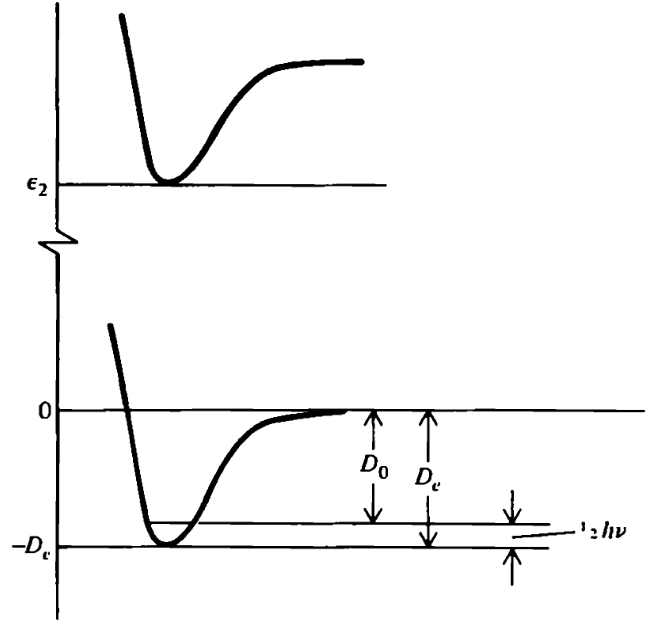
\includegraphics[width=0.7\linewidth]{electronic_states.png}
	\caption{Electronic potentials for the ground and first excited state with
	relevant quantities marked.}
	\label{fig:diatomicelectronic}
\end{figure}

\subsection{Deriving the Partition Function}
In order to derive the partition function, a zero state energy must be assigned.
Two possibilities exist 0 or $h\nu/2$. The book uses the latter and so shall I.
The derivation of the vibrational partition function goes as follows,
\begin{align*}
	q_{vib} &= \sum_{n}{e^{-\beta\epsilon_n}}\\
			&= \sum_{n}{e^{-\beta h\nu(n+1/2)}} = \sum_{n}{e^{-\beta h\nu
			n}e^{-\beta h\nu/2}}\\
			&= e^{-\beta h\nu/2}\sum_{n=0}^{\infty}{e^{-\beta h \nu n}}\\
			&= \frac{e^{-\beta h\nu/2}}{1 - e^{-\beta h \nu}} \qquad e^{-\beta h
			\nu} < 1.
\end{align*}
The first step follows by definition. The second is just the expansion and
simplification of $\epsilon_{vib}$. The third is just taking the constant out of
the sum. The fourth step involves seeing that the sum is a geometric series if
$e^{-\beta h \nu} < 1$. The partition function here is exact given the
constraint, but we can still take a high temperature limit using an integral.
This then is,
\begin{equation*}
	q_{vib} = e^{-\beta h\nu/2}\int_{n=0}^{\infty}{e^{-\beta h \nu n}\d n}
	= \frac{kT}{h\nu}.
\end{equation*}
\subsection{Properties of Vibrational Mode}
We will look at level occupancy and average vibrational energy. The average
energy given by the exact partition function is,
\begin{align*}
	E_v &= NkT^2 \frac{\d\ln q_v}{\d T} = NkT^2\frac{\d}{\d T}
	\left(\frac{h\nu}{2kT} - \ln{(1 - e^{-h\nu/kT})}\right)\\
		&= \frac{Nk\Theta}{2} + Nk\Theta \frac{e^{-\Theta/T}}{1 -
			e^{-\Theta/T}} = Nk\Theta \left(\frac{1}{2} + \frac{1}{e^{\Theta/T}
		-1}\right).
\end{align*}
Where, $\Theta = h\nu/k$. For the high temperature limit, we have,
\begin{equation*}
	E_v = NkT^2 \frac{\d\ln q_v}{\d T} = NkT^2 \frac{\d}{\d
	T}\left(\ln{\frac{T}{\Theta}}\right) = NkT.
\end{equation*}
The specific heat in this case is simply $Nk$ since $C_v$ is the derivative of
energy with respect to temperature.

The fraction of molecules in a given energy state are,
\begin{equation*}
	f_n = \frac{e^{-\beta h\nu (n+1/2)}}{q_{vib}}.
\end{equation*}
Therefore the fraction of molecules in an excited state are,
\begin{equation*}
	f_{n > 0} = \frac{\sum_{n=1}^{\infty}{e^{-\beta h\nu (n+1/2)}}}{q_{vib}} = 1
	- f_0 = \frac{e^{-\beta h\nu /2}}{q_{vib}} = 1 - (1 - e^{-\beta h \nu}) =
	e^{-\beta h \nu}.
\end{equation*}
The solution comes from the fact that the fraction in a excited state is the
inverse of the fraction in the ground state.

\section{Rotational Partition Function}%
\subsection{Energy States and Spectra}
\label{sec:rot}
For a rigid rotor the energy states and degeneracy are given by,
\begin{align*}
	\epsilon_j &= \frac{\hbar^2 J(J+1)}{2 I}\\
	\omega_j &= 2J+1.
\end{align*}
Here, $I$ is the moment of inertia, which is $\mu r_e^2 $ for the diatomic
case. $\mu$ is the reduced mass of the molecule. 

The transition rules for rotational energy are that the transition must be
adjacent like the vibrational modes and the molecule must have a permanent
dipole moment. The electromagnetic spectra that comes from the rotational energy
is then given by taking the different in adjacent energy levels like before.
\begin{align*}
	\Delta\epsilon &= \epsilon_{j+1} - \epsilon_j = \frac{\hbar^2}{2I} ((J+1)(J+2)
	- J(J+1)) = \frac{\hbar^2}{I} (J+1)\\
	\nu &= \frac{\Delta\epsilon}{h} = \frac{h}{4\pi^2 I}(J+1)
\end{align*}
To get the final form, $\hbar$ was expanded to $h/2\pi$. What this says is
unlike vibrational energy, rotational energy transitions emit multiple
wavelengths. \note we will set the rotational ground energy to zero.

\subsection{Deriving the Rotational Partition Function}
\subsection{Heteronuclear Derivation}
For reasons of wavefunction symmetry under the exchange of particles we must
separate the heteronuclear and homonuclear cases. We begin by examining the
heteronuclear.

By definition,
\begin{equation*}
	q_{rot} = \sum_{J=0}^{\infty}{(2J+1)e^{-\beta\bar{B}J(J+1)}}.
\end{equation*}
The variable $\bar{B}$ is $h/8\pi^2 Ic$ where c is the speed of light. Then,
$\epsilon_J = \bar{B}J(J+1)$. We can further define $\Theta_r$ to be $\bar{B}/k$
which is a rotational temperature. In order to write the summation in terms of a
integral we require that the difference between adjacent values be small. This
is fulfilled if $\Theta_r / k (J+1)$ is small which is true at small $J$. By the
time large $J$ are reached the contributions become negligible though, so we can
just take the integral.
\begin{align*}
	q_{rot} &= \int_0^{\infty}{(2J+1) e^{-\Theta_r J(J+1)/T} \d J}\\
			&= \int_0^{\infty}{e^{-\Theta_r J(J+1)/T} \d [J(J+1)]} = \left[
			\frac{T}{\Theta_r} e^{-\Theta_r J(J+1)/T}\right]_{0}^{\infty} =
			\frac{T}{\Theta_r}\\
			&= \frac{8\pi^2 IkT}{h^{2}}. 
\end{align*}
The second line recognizes that a change of variable can drastically simplify
the integral. For cases where the above is a bad approximation say $\Theta_r >
0.7T$, the summation can be expanded to 4 terms with good accuracy. Of course
higher order approximations can be taken.

The two approximation, however, leave an intermediate gap. The solution is to
use a Euler-MacLaurin summation formula approximation. This is given by
\begin{equation*}
	\sum_{n=a}^{b}{f(n)} = \int_{a}^{b}{f(n)\d n} + \frac{1}{2} [f(b)+f(a)] +
			\sum_{j=1}^{\infty}(-1)^{j}\frac{B_j}{(2j)!}[f^{(2j-1)}(a) -
			f^{(2j-1)}(b)],
\end{equation*}
where $B_j$ is the $j$-th Bernoulli number and the last bracketed term uses the
$(2j-1)$-th derivative. This give for the rotational partition function,
\begin{equation*}
	q_{rot} = \frac{T}{\Theta_r} \left( 1 +
		\frac{1}{3}\left(\frac{\Theta_r}{T}\right) +
		\frac{1}{15}\left(\frac{\Theta_r}{T}\right)^2 +
	\frac{1}{315}\left(\frac{\Theta_r}{T}\right)^3 + \cdots\right).
\end{equation*}

\subsection{Heteronuclear Thermodynamics}
The ensemble rotational energy in the high temperature limit is,
\begin{equation*}
	E_r = NkT^2 \left(\frac{\partial \ln q_{rot}}{\partial T}\right) = NkT^2
	\left(\frac{\partial}{\partial T}\right) (\ln T - \ln \Theta_r) = NkT.
\end{equation*}
This means that $C_v$ like in the vibrational case is $Nk$. The fraction of
molecules in a particular vibrational state can be taken just like the
rotational state, but since it is an identical procedure it is not shown here.
However, an important feature of rotational energy levels is that the most
occupied level at room temperature is an excited state. The most occupied level
can be derived by taking the derivative of the occupancy fraction,
\begin{equation*}
	\frac{\d f_J}{\d J} = \frac{\d}{\d J}\left(\frac{N_J}{N}\right) =
	\frac{\d}{\d J}\left(\frac{(2J+1)e^{-\Theta_r J(J+1)/T}}{q_{rot}}\right),
\end{equation*}
and setting it equal to zero.

\subsection{Homonuclear Derivation}
\note The homonuclear case can be approximated by
\begin{equation*}
	q_{rot,homo} = \frac{q_{rot,heter}}{2}.
\end{equation*}
This deals with the fact that in the homonuclear case a two-fold symmetry exists
perpendicular to the interatomic axis. This prevents the over counting of states.
This factor of 2 can be generalized to a factor $\sigma$ which is called the
symmetry number and represents the number of indistinguishable rotational states
or the number or rotational symmetries.

However, this will not work at low temperatures since homonuclear diatomic
molecules must obey certain wavefunction symmetries when an exchange of nuclei
is performed. This symmetry depends on the spins of the nuclei. If the spins are
integers the wavefunction is symmetric; otherwise, the wavefunction is
anti-symmetric with respect to exchange.

\subsubsection{Digression on Symmetry Requirements}
To determine the individual symmetry contributions of the electronic,
translational, vibrational, rotational, and nuclear energies to the
wavefunction, we imagine that we take a diatomic molecule and exchange both
nuclei along with their electrons. We then flip the electrons again. For
molecules where only the ground electronic state is useful and ground state is
$\Sigma_g^+$, the electronic wavefunction is symmetric to such operations. The
translational and vibration wavefunctions are obviously unaffected by such
transformations. This only leaves the nuclear and rotational.

By looking at the rotational wavefunctions for hydrogen, one can see that even
$J$ are symmetric to the swap, but odd $J$ are anti-symmetric to it. In
addition, for hydrogen, the nuclei spins are $\pm 1/2$. This leads to four spin
combinations: three are symmetric and one is anti-symmetric. Since the total
wavefunction must be anti-symmetric we must pair symmetric rotational
wavefunctions with anti-symmetric nuclear wavefunctions and vice versa. The
opposite holds true for integer spin molecules.

For a generic system the number of spin states for a nucleus is $2I+1$. For a
diatomic molecule there are $(2I+1)^2$ states then. The number of antisymmetric
states can be calculated using $(2I+1)(2I)/2$. The number of symmetric is just
the total minus the number of antisymmetric wavefunctions. This leads to
\begin{itemize}
	\item Integral spin
		\begin{itemize}
			\item Odd J - I(2I+1)
			\item Even J - (I+1)(2I+1)
		\end{itemize}
	\item Half-integral spin
		\begin{itemize}
			\item Odd J - (I+1)(2I+1)
			\item Even J - I(2I+1).
		\end{itemize}
\end{itemize}
One can see that the two are just mirrors of each other. The partition function
is then,
\begin{equation*}
	q_{rot,nucl} = w_{k,even}\sum_{J~even}{(2J+1)e^{-\Theta_r J(J+1)/T}} +
	w_{k,odd}\sum_{J~odd}{(2J+1)e^{-\Theta_r J(J+1)/T}},
\end{equation*}
where $w_{k,even/odd}$ represents the appropriate spin weighting. The rotation
and nuclear partition functions are then coupled. However, at high temperatures,
\begin{equation*}
	\sum_{J~odd} \approx \sum_{J~even} \approx \frac{1}{2}\sum_{J}.
\end{equation*}
This is just one half of the heteronuclear case. Then all the previous equations
apply with the adding factor of $1/2$. In this limit, we can separate the
partition functions to get,
\begin{align*}
	q_{rot} &= \frac{T}{2\Theta_r} = \frac{T}{\sigma\Theta_r}\\
	q_{nucl} &= (2I+1)^2.
\end{align*}
This requires that $\Theta_r < 0.2T$. $\sigma$ is just the symmetry number
mentioned previously. When the temperature is not high enough however the
coupled partition function must be used. In general, this is only necessary with
molecules like hydrogen where $\Theta_r$ is appreciable at gas temperatures. The
splitting of $H_2$ into two different types para (parallel spins) and ortho
(anti-parallel spins) comes from this weighting. At room temperature $H_2$ is
25\% para and 75\% ortho. At lower temperatures though this ratio changes as the
summations over even and odd $J$'s are not approximately equivalent.

All thermodynamic quantities can be calculated normally and will either not vary
in the high temperature limit (as is the case for energy and specific heat) or
will vary by factors of $\sigma$. This is also true in the Euler-MacLaurin
approximation.

\section{Total Partition Function}%
\label{sec:tpf}
The total partition function then becomes at the high temperature limit of the
harmonic-oscillator rigid rotor approximation,
\begin{align*}
	q &= q_{trans}~q_{rot}~q_{vib}~q_{nucl}~q_{elec}\\
	  &= \left(\frac{2\pi mkT}{h^2 }\right)^{3/2} V \frac{8\pi^2 IkT}{\sigma
	  h^{2}} \frac{e^{-\beta h\nu/2}}{1 - e^{-\beta h\nu}} \omega_{e1}
		  e^{D_e/kT}.
\end{align*}
This equation ignores the nuclear partition function.

\note In cases where the ground electronic state is not a $\Sigma$ state, the
electronic and nuclear angular momentum must be coupled. At high temperatures
compared to $\Theta_r$, they can still be decoupled, however. This means that
for all but low temperatures for molecules like NO the previous approach would
work.
